\batchmode
\documentclass{book}
\usepackage[a4paper,top=2.5cm,bottom=2.5cm,left=2.5cm,right=2.5cm]{geometry}
\usepackage{makeidx}
\usepackage{natbib}
\usepackage{graphicx}
\usepackage{multicol}
\usepackage{float}
\usepackage{listings}
\usepackage{color}
\usepackage{ifthen}
\usepackage[table]{xcolor}
\usepackage{textcomp}
\usepackage{alltt}
\usepackage[utf8]{inputenc}
\usepackage{mathptmx}
\usepackage[scaled=.90]{helvet}
\usepackage{courier}
\usepackage{sectsty}
\usepackage{amssymb}
\usepackage[titles]{tocloft}
\usepackage{doxygen}
\lstset{language=C++,inputencoding=utf8,basicstyle=\footnotesize,breaklines=true,breakatwhitespace=true,tabsize=8,numbers=left }
\makeindex
\setcounter{tocdepth}{3}
\renewcommand{\footrulewidth}{0.4pt}
\renewcommand{\familydefault}{\sfdefault}
\hfuzz=15pt
\setlength{\emergencystretch}{15pt}
\hbadness=750
\tolerance=750
\begin{document}
\begin{titlepage}
\vspace*{7cm}
\begin{center}
{\Large Grijper }\\
\vspace*{1cm}
{\large Generated by Doxygen 1.8.3.1}\\
\vspace*{0.5cm}
{\small Tue Sep 24 2013 15:54:29}\\
\end{center}
\end{titlepage}
\clearemptydoublepage
\pagenumbering{roman}
\tableofcontents
\clearemptydoublepage
\pagenumbering{arabic}
\chapter{Main Page}
\label{index} \section*{\doxyref{Grijper}{p.}{namespaceGrijper}}

\subsection*{Controlling a robotic hand}

{\bfseries \doxyref{Grijper}{p.}{namespaceGrijper}} is a package containing nodes that are used to control a motorised robotic hand, henceforth called the 'gripper'.

{\ttfamily This} is done by reading and evaluating a sensor and it's values using the phidget in the phidget\-\_\-reader node. These are compared to set threshold values to decide if the gripper should be opened or closed. This is done in the controller. Commands are then sent to the actuator which controlls the motor powering the gripper. This actuator node then publishes the motor state.

{\ttfamily This} state is picked up by an rviz node that visualises and controls the gripper model in rviz. The state is given as a float between 0.\-0 and 1.\-0. 0.\-0 indicating the gripper is completely open and 1.\-0 indicates the gripper has been closed. Another rviz node listens to the phidget sensor values and visualises a cyllinder mimicking the position of the oject relative to the gripper.\section{R\-O\-S Grijper A\-P\-I}\label{index_rosapi}
List of nodes\-:
\begin{DoxyItemize}
\item {\bfseries }[gripper\-\_\-console]\-: gripper\-\_\-\-\_\-console\-\_\-8cpp.\-html
\item {\bfseries }[gripper\-\_\-controller]\-: ./gripper\-\_\-\-\_\-controller\-\_\-8cpp.html
\item {\bfseries }[gripper\-\_\-actuator]\-: ./gripper\-\_\-\-\_\-actuator\-\_\-8cpp.html
\item {\bfseries }[phidget\-\_\-reader]\-: ./phidget\-\_\-\-\_\-reader\-\_\-8cpp.html
\item {\bfseries }[rviz\-\_\-gripper]\-: ./rviz\-\_\-\-\_\-gripper\-\_\-8cpp.html
\item {\bfseries }[rviz\-\_\-object]\-: ./rviz\-\_\-\-\_\-object\-\_\-8cpp.html
\end{DoxyItemize}



\subsection{gripper\-\_\-console}\label{index_node_name}
node\-\_\-name makes the system controllable by the user through console input and output.\subsubsection{Usage}\label{index_Usage}
\begin{DoxyVerb}$ node_type1 [standard ROS args]
\end{DoxyVerb}


\begin{DoxyParagraph}{Example}

\end{DoxyParagraph}
\begin{DoxyVerb}$ node_type1
\end{DoxyVerb}
\subsubsection{R\-O\-S topics}\label{index_topics}
Subscribes to\-:
\begin{DoxyItemize}
\item {\bfseries \char`\"{}in\char`\"{}}\-: [std\-\_\-msgs/\-Foo\-Type] description of in
\end{DoxyItemize}

Publishes to\-:
\begin{DoxyItemize}
\item {\bfseries \char`\"{}out\char`\"{}}\-: [std\-\_\-msgs/\-Foo\-Type] description of out
\end{DoxyItemize}\subsubsection{R\-O\-S parameters}\label{index_parameters}
Reads the following parameters from the parameter server


\begin{DoxyItemize}
\item {\bfseries \char`\"{}$\sim$param\-\_\-name\char`\"{}} \-: {\bfseries }[type] description of param\-\_\-name
\item {\bfseries \char`\"{}$\sim$my\-\_\-param\char`\"{}} \-: {\bfseries }[string] description of my\-\_\-param
\end{DoxyItemize}

Sets the following parameters on the parameter server


\begin{DoxyItemize}
\item {\bfseries \char`\"{}$\sim$param\-\_\-name\char`\"{}} \-: {\bfseries }[type] description of param\-\_\-name
\end{DoxyItemize}\subsubsection{R\-O\-S services}\label{index_services}

\begin{DoxyItemize}
\item {\bfseries \char`\"{}foo\-\_\-service\char`\"{}}\-: [std\-\_\-srvs/\-Foo\-Type] description of foo\-\_\-service
\end{DoxyItemize}\section{Command-\/line tools}\label{index_commandline}
This section is a catch-\/all for any additional tools that your package provides or uses that may be of use to the reader. For example\-:


\begin{DoxyItemize}
\item tools/scripts (e.\-g. rospack, roscd)
\item roslaunch .launch files
\item xmlparam files
\end{DoxyItemize}\subsection{script\-\_\-name}\label{index_script_name}
Description of what this script/file does.\subsubsection{Usage}\label{index_Usage}
\begin{DoxyVerb}$ ./script_name [args]
\end{DoxyVerb}


\begin{DoxyParagraph}{Example}

\end{DoxyParagraph}
\begin{DoxyVerb}$ ./script_name foo bar
\end{DoxyVerb}
 
\chapter{File Index}
\section{File List}
Here is a list of all files with brief descriptions\-:\begin{DoxyCompactList}
\item\contentsline{section}{{\bf \-\_\-\-\_\-init\-\_\-\-\_\-.\-py} }{\pageref{____init_____8py}}{}
\item\contentsline{section}{{\bf msg/\-\_\-\-\_\-init\-\_\-\-\_\-.\-py} }{\pageref{msg_2____init_____8py}}{}
\item\contentsline{section}{{\bf \-\_\-command.\-py} }{\pageref{__command_8py}}{}
\item\contentsline{section}{{\bf command.\-h} }{\pageref{command_8h}}{}
\item\contentsline{section}{{\bf console.\-cpp} }{\pageref{console_8cpp}}{}
\item\contentsline{section}{{\bf gripper\-\_\-actuator.\-cpp} }{\pageref{gripper__actuator_8cpp}}{}
\item\contentsline{section}{{\bf gripper\-\_\-controller.\-cpp} }{\pageref{gripper__controller_8cpp}}{}
\item\contentsline{section}{{\bf phidget\-\_\-reader.\-cpp} }{\pageref{phidget__reader_8cpp}}{}
\item\contentsline{section}{{\bf rviz\-\_\-gripper.\-cpp} }{\pageref{rviz__gripper_8cpp}}{}
\item\contentsline{section}{{\bf rviz\-\_\-object.\-cpp} }{\pageref{rviz__object_8cpp}}{}
\end{DoxyCompactList}

\chapter{File Documentation}
\section{gripper\-\_\-actuator.\-cpp File Reference}
\label{gripper__actuator_8cpp}\index{gripper\-\_\-actuator.\-cpp@{gripper\-\_\-actuator.\-cpp}}
{\ttfamily \#include $<$ros/ros.\-h$>$}\\*
{\ttfamily \#include $<$string$>$}\\*
{\ttfamily \#include $<$std\-\_\-msgs/\-Float32.\-h$>$}\\*
{\ttfamily \#include $<$std\-\_\-msgs/\-String.\-h$>$}\\*
{\ttfamily \#include $<$std\-\_\-msgs/\-Bool.\-h$>$}\\*
{\ttfamily \#include $<$Grijper/command.\-h$>$}\\*
{\ttfamily \#include $<$threemxl/\-C3mxl\-R\-O\-S.\-h$>$}\\*
Include dependency graph for gripper\-\_\-actuator.\-cpp\-:\nopagebreak
\begin{figure}[H]
\begin{center}
\leavevmode
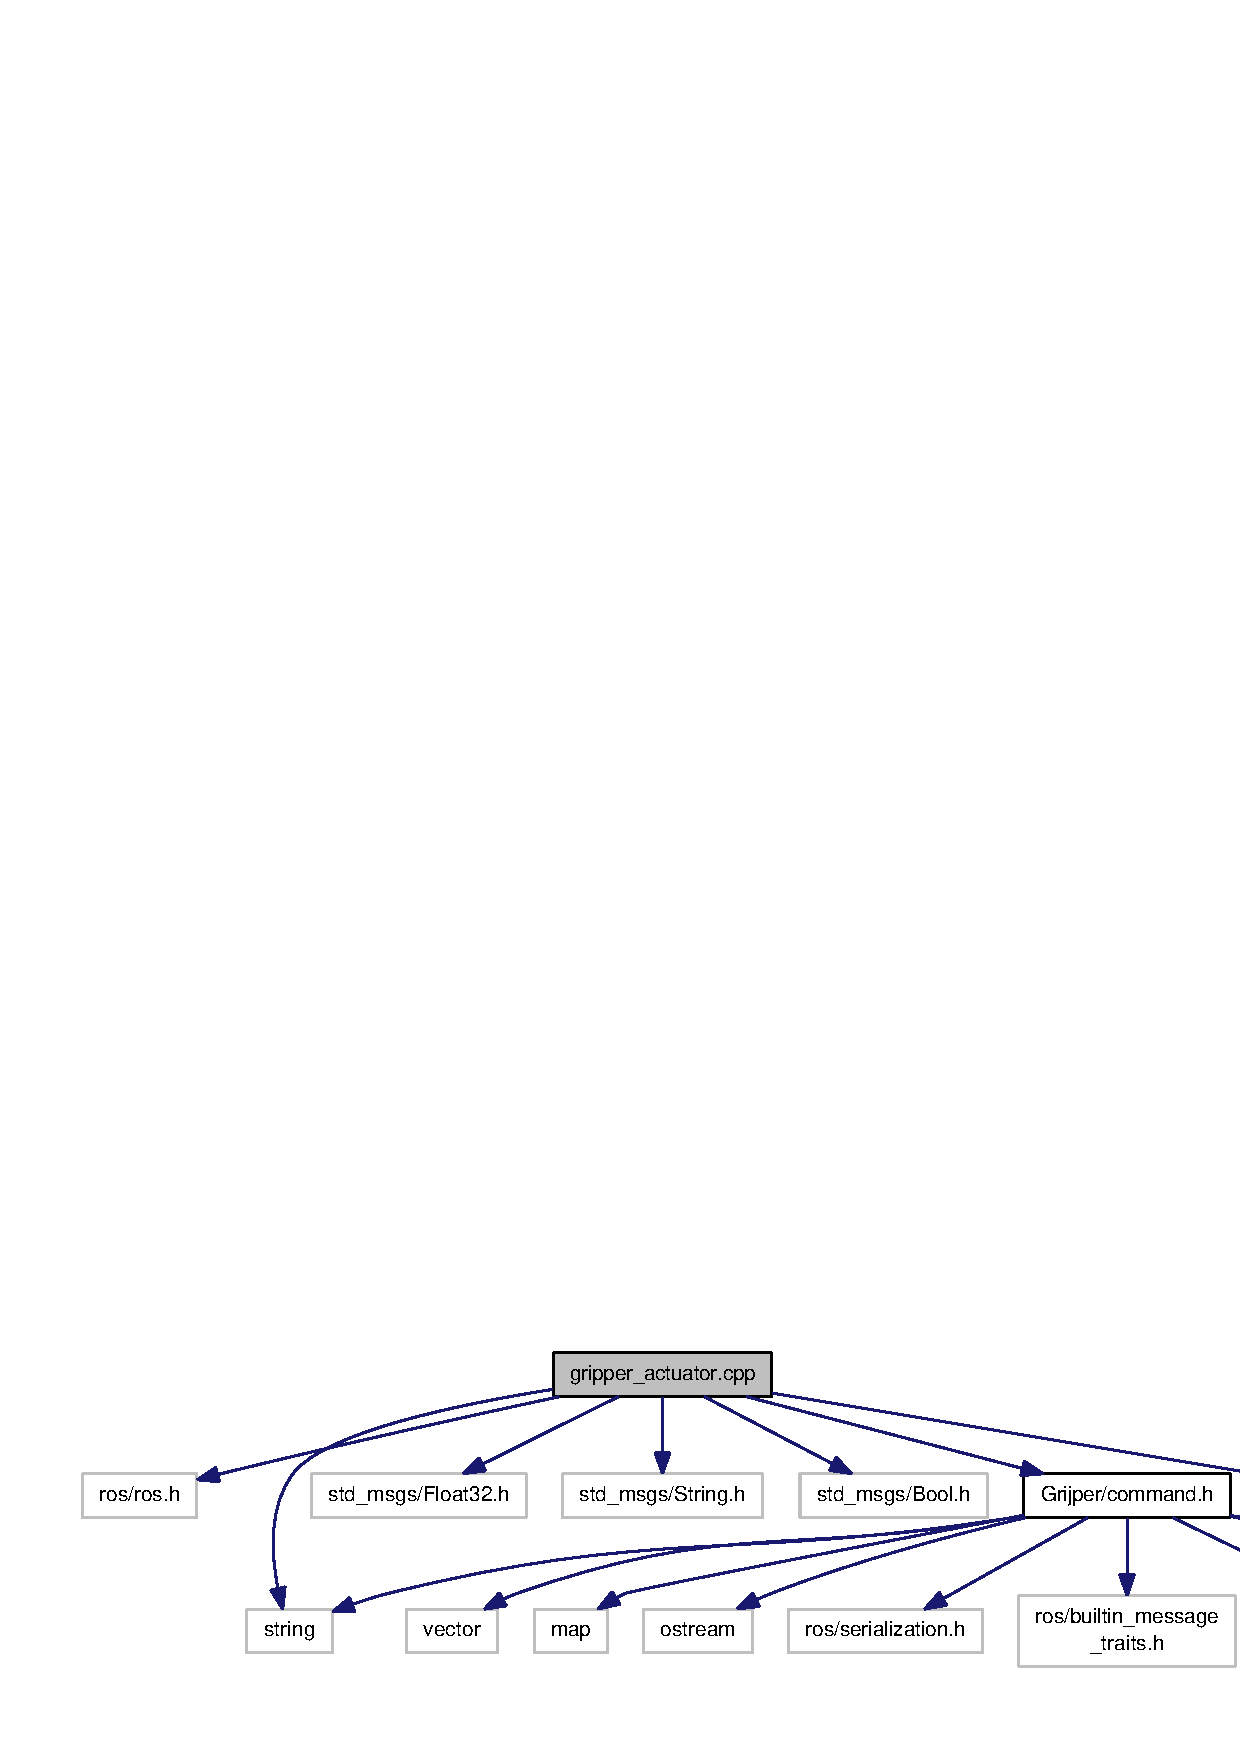
\includegraphics[width=350pt]{gripper__actuator_8cpp__incl}
\end{center}
\end{figure}
\subsection*{Functions}
\begin{DoxyCompactItemize}
\item 
float {\bf calc\-\_\-current} (float {\bf force})
\begin{DoxyCompactList}\small\item\em Conversion method to convert a target force into a current. \end{DoxyCompactList}\item 
bool {\bf close} ()
\begin{DoxyCompactList}\small\item\em Small controlling method for closing the gripper. \end{DoxyCompactList}\item 
void {\bf gripper\-Control} (const {\bf Grijper\-::command\-::\-Const\-Ptr} \&msg)
\begin{DoxyCompactList}\small\item\em This method controls the motor. \end{DoxyCompactList}\item 
int {\bf main} (int argc, char $\ast$$\ast$argv)
\begin{DoxyCompactList}\small\item\em Main method of this node. All commands are evaluated here, and motor actuation is controlled from here. \end{DoxyCompactList}\item 
bool {\bf open} ()
\begin{DoxyCompactList}\small\item\em Small controlling method for opening the gripper. \end{DoxyCompactList}\item 
bool {\bf relax} ()
\begin{DoxyCompactList}\small\item\em Small controlling method for relaxing the gripper. \end{DoxyCompactList}\item 
void {\bf shutdown} (const std\-\_\-msgs\-::\-Bool\-::\-Const\-Ptr \&b)
\begin{DoxyCompactList}\small\item\em Controll method to shutdown this R\-O\-S node when the command is given. \end{DoxyCompactList}\end{DoxyCompactItemize}
\subsection*{Variables}
\begin{DoxyCompactItemize}
\item 
float {\bf current} = 0.\-04
\item 
ros\-::\-Publisher {\bf gripper\-\_\-state}
\item 
C\-Dxl\-Generic $\ast$ {\bf motor\-\_\-}
\end{DoxyCompactItemize}


\subsection{Function Documentation}
\index{gripper\-\_\-actuator.\-cpp@{gripper\-\_\-actuator.\-cpp}!calc\-\_\-current@{calc\-\_\-current}}
\index{calc\-\_\-current@{calc\-\_\-current}!gripper_actuator.cpp@{gripper\-\_\-actuator.\-cpp}}
\subsubsection[{calc\-\_\-current}]{\setlength{\rightskip}{0pt plus 5cm}float calc\-\_\-current (
\begin{DoxyParamCaption}
\item[{float}]{force}
\end{DoxyParamCaption}
)}\label{gripper__actuator_8cpp_a9b3c7d64d58f6a1d4a9f53a6e4a3aa27}


Conversion method to convert a target force into a current. 

Converts a target force into a current that can be passed on to the motor. 
\begin{DoxyParams}{Parameters}
{\em force} & The target force as a float. \\
\hline
\end{DoxyParams}
\begin{DoxyReturn}{Returns}
The calculated current. 
\end{DoxyReturn}


Definition at line 119 of file gripper\-\_\-actuator.\-cpp.

\index{gripper\-\_\-actuator.\-cpp@{gripper\-\_\-actuator.\-cpp}!close@{close}}
\index{close@{close}!gripper_actuator.cpp@{gripper\-\_\-actuator.\-cpp}}
\subsubsection[{close}]{\setlength{\rightskip}{0pt plus 5cm}bool close (
\begin{DoxyParamCaption}
{}
\end{DoxyParamCaption}
)}\label{gripper__actuator_8cpp_a46143fd6de3be9ab9951f140d3ae8c2f}


Small controlling method for closing the gripper. 

This method closes the gripper with the corresponding force. \begin{DoxyReturn}{Returns}
True 
\end{DoxyReturn}


Definition at line 96 of file gripper\-\_\-actuator.\-cpp.

\index{gripper\-\_\-actuator.\-cpp@{gripper\-\_\-actuator.\-cpp}!gripper\-Control@{gripper\-Control}}
\index{gripper\-Control@{gripper\-Control}!gripper_actuator.cpp@{gripper\-\_\-actuator.\-cpp}}
\subsubsection[{gripper\-Control}]{\setlength{\rightskip}{0pt plus 5cm}void gripper\-Control (
\begin{DoxyParamCaption}
\item[{const {\bf Grijper\-::command\-::\-Const\-Ptr} \&}]{msg}
\end{DoxyParamCaption}
)}\label{gripper__actuator_8cpp_add43683f423b8ad34526564c0760d596}


This method controls the motor. 

This method is called every time a command from the controller has been given. This command is evaluated and executed. The msg parameter contains the 'cmd' string describing the command to be executed and also a 'force' float that indicates the target force. This target force is converted to a current, which is passed in to the motor, with a sign and magnitude according to the command.


\begin{DoxyParams}{Parameters}
{\em msg} & The message containing the command and target force. \\
\hline
\end{DoxyParams}


Definition at line 63 of file gripper\-\_\-actuator.\-cpp.

\index{gripper\-\_\-actuator.\-cpp@{gripper\-\_\-actuator.\-cpp}!main@{main}}
\index{main@{main}!gripper_actuator.cpp@{gripper\-\_\-actuator.\-cpp}}
\subsubsection[{main}]{\setlength{\rightskip}{0pt plus 5cm}int main (
\begin{DoxyParamCaption}
\item[{int}]{argc, }
\item[{char $\ast$$\ast$}]{argv}
\end{DoxyParamCaption}
)}\label{gripper__actuator_8cpp_a3c04138a5bfe5d72780bb7e82a18e627}


Main method of this node. All commands are evaluated here, and motor actuation is controlled from here. 

This method controls the motor powering the gripper. This also meand publishing the gripper state when it has changed.

This node also listens to the shutdown command given by the controller. 

Definition at line 28 of file gripper\-\_\-actuator.\-cpp.

\index{gripper\-\_\-actuator.\-cpp@{gripper\-\_\-actuator.\-cpp}!open@{open}}
\index{open@{open}!gripper_actuator.cpp@{gripper\-\_\-actuator.\-cpp}}
\subsubsection[{open}]{\setlength{\rightskip}{0pt plus 5cm}bool open (
\begin{DoxyParamCaption}
{}
\end{DoxyParamCaption}
)}\label{gripper__actuator_8cpp_adb20eae91802d6ad6366cdee0220c280}


Small controlling method for opening the gripper. 

This method opens the gripper with the corresponding force. \begin{DoxyReturn}{Returns}
True 
\end{DoxyReturn}


Definition at line 85 of file gripper\-\_\-actuator.\-cpp.

\index{gripper\-\_\-actuator.\-cpp@{gripper\-\_\-actuator.\-cpp}!relax@{relax}}
\index{relax@{relax}!gripper_actuator.cpp@{gripper\-\_\-actuator.\-cpp}}
\subsubsection[{relax}]{\setlength{\rightskip}{0pt plus 5cm}bool relax (
\begin{DoxyParamCaption}
{}
\end{DoxyParamCaption}
)}\label{gripper__actuator_8cpp_a76ee232c68955d5e8c9e507b8ac38436}


Small controlling method for relaxing the gripper. 

This method relaxed the gripper. \begin{DoxyReturn}{Returns}
True 
\end{DoxyReturn}


Definition at line 107 of file gripper\-\_\-actuator.\-cpp.

\index{gripper\-\_\-actuator.\-cpp@{gripper\-\_\-actuator.\-cpp}!shutdown@{shutdown}}
\index{shutdown@{shutdown}!gripper_actuator.cpp@{gripper\-\_\-actuator.\-cpp}}
\subsubsection[{shutdown}]{\setlength{\rightskip}{0pt plus 5cm}void shutdown (
\begin{DoxyParamCaption}
\item[{const std\-\_\-msgs\-::\-Bool\-::\-Const\-Ptr \&}]{b}
\end{DoxyParamCaption}
)}\label{gripper__actuator_8cpp_a6099bcde46c020c0703be2c28a4432d5}


Controll method to shutdown this R\-O\-S node when the command is given. 

This method will shutdown this node when the command is given by the console. 
\begin{DoxyParams}{Parameters}
{\em b} & The message containing the command. Nothing is done with the command since we know what it will be when this message is received. \\
\hline
\end{DoxyParams}


Definition at line 128 of file gripper\-\_\-actuator.\-cpp.



\subsection{Variable Documentation}
\index{gripper\-\_\-actuator.\-cpp@{gripper\-\_\-actuator.\-cpp}!current@{current}}
\index{current@{current}!gripper_actuator.cpp@{gripper\-\_\-actuator.\-cpp}}
\subsubsection[{current}]{\setlength{\rightskip}{0pt plus 5cm}float current = 0.\-04}\label{gripper__actuator_8cpp_af9653d31acfffa5a40aa709b2065e00b}
Target current variable, default is set to 0.\-04. 

Definition at line 18 of file gripper\-\_\-actuator.\-cpp.

\index{gripper\-\_\-actuator.\-cpp@{gripper\-\_\-actuator.\-cpp}!gripper\-\_\-state@{gripper\-\_\-state}}
\index{gripper\-\_\-state@{gripper\-\_\-state}!gripper_actuator.cpp@{gripper\-\_\-actuator.\-cpp}}
\subsubsection[{gripper\-\_\-state}]{\setlength{\rightskip}{0pt plus 5cm}ros\-::\-Publisher gripper\-\_\-state}\label{gripper__actuator_8cpp_a9f4419e4ba603a6e5cbe0148e492cad0}
Gripper state publisher. 

Definition at line 12 of file gripper\-\_\-actuator.\-cpp.

\index{gripper\-\_\-actuator.\-cpp@{gripper\-\_\-actuator.\-cpp}!motor\-\_\-@{motor\-\_\-}}
\index{motor\-\_\-@{motor\-\_\-}!gripper_actuator.cpp@{gripper\-\_\-actuator.\-cpp}}
\subsubsection[{motor\-\_\-}]{\setlength{\rightskip}{0pt plus 5cm}C\-Dxl\-Generic$\ast$ motor\-\_\-}\label{gripper__actuator_8cpp_ac1874704ed544a18b8fc45cd2abacecc}
Threemxl generic motor controller pointer. 

Definition at line 19 of file gripper\-\_\-actuator.\-cpp.


\section{gripper\-\_\-controller.\-cpp File Reference}
\label{gripper__controller_8cpp}\index{gripper\-\_\-controller.\-cpp@{gripper\-\_\-controller.\-cpp}}
{\ttfamily \#include $<$ros/ros.\-h$>$}\\*
{\ttfamily \#include $<$cmath$>$}\\*
{\ttfamily \#include $<$string$>$}\\*
{\ttfamily \#include $<$std\-\_\-msgs/\-Float32.\-h$>$}\\*
{\ttfamily \#include $<$std\-\_\-msgs/\-Bool.\-h$>$}\\*
{\ttfamily \#include $<$std\-\_\-msgs/\-String.\-h$>$}\\*
{\ttfamily \#include $<$Grijper/command.\-h$>$}\\*
Include dependency graph for gripper\-\_\-controller.\-cpp\-:\nopagebreak
\begin{figure}[H]
\begin{center}
\leavevmode
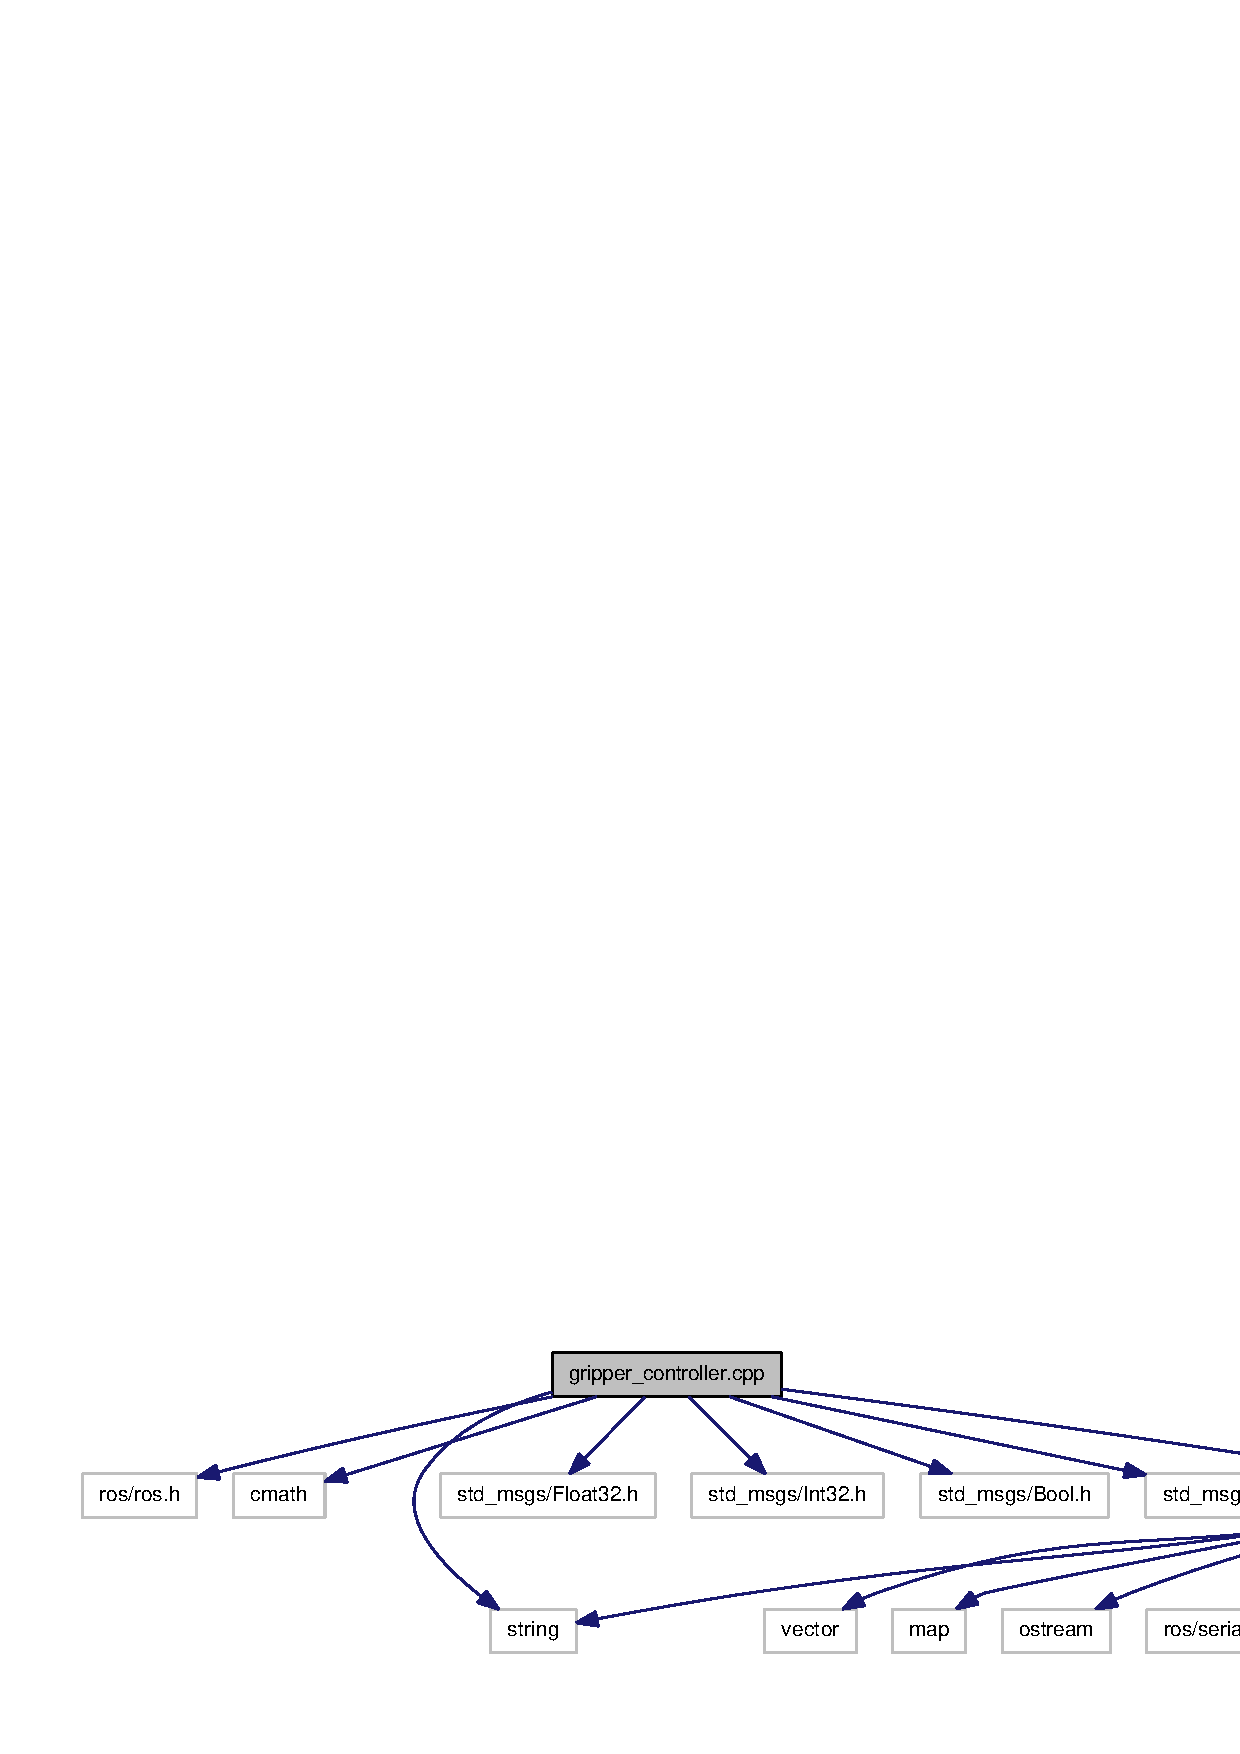
\includegraphics[width=350pt]{gripper__controller_8cpp__incl}
\end{center}
\end{figure}
\subsection*{Functions}
\begin{DoxyCompactItemize}
\item 
bool {\bf close\-\_\-gripper} (float distance)
\begin{DoxyCompactList}\small\item\em Small evaluation method to see if the gripper should be closed. \end{DoxyCompactList}\item 
void {\bf gripper\-Command} (const std\-\_\-msgs\-::\-String\-::\-Const\-Ptr \&msg)
\begin{DoxyCompactList}\small\item\em Method for evaluating and executing commands received from the console. \end{DoxyCompactList}\item 
void {\bf gripper\-Phidget} (const std\-\_\-msgs\-::\-Float32\-::\-Const\-Ptr \&msg)
\begin{DoxyCompactList}\small\item\em Method that evaluates the phidget sensor values and takes appropriate action. \end{DoxyCompactList}\item 
int {\bf main} (int argc, char $\ast$$\ast$argv)
\begin{DoxyCompactList}\small\item\em Main method of the controller node. All incoming messages are analysed and commands are sent from this node. \end{DoxyCompactList}\item 
bool {\bf open\-\_\-gripper} (float distance)
\begin{DoxyCompactList}\small\item\em Small evaluation method to see if the gripper should be opened. \end{DoxyCompactList}\item 
void {\bf set\-Force} (const std\-\_\-msgs\-::\-Float32\-::\-Const\-Ptr \&msg)
\begin{DoxyCompactList}\small\item\em Method for setting the force on message receiving. \end{DoxyCompactList}\item 
void {\bf shutdown} (const std\-\_\-msgs\-::\-Bool\-::\-Const\-Ptr \&b)
\begin{DoxyCompactList}\small\item\em Controll method to shutdown this R\-O\-S node when the command is given. \end{DoxyCompactList}\end{DoxyCompactItemize}
\subsection*{Variables}
\begin{DoxyCompactItemize}
\item 
ros\-::\-Publisher {\bf control}
\item 
float {\bf force} = 0.\-35
\item 
bool {\bf force\-\_\-open} = false
\item 
bool {\bf gripper\-\_\-open} = true
\item 
float {\bf last\-\_\-distance} = 0
\end{DoxyCompactItemize}


\subsection{Function Documentation}
\index{gripper\-\_\-controller.\-cpp@{gripper\-\_\-controller.\-cpp}!close\-\_\-gripper@{close\-\_\-gripper}}
\index{close\-\_\-gripper@{close\-\_\-gripper}!gripper_controller.cpp@{gripper\-\_\-controller.\-cpp}}
\subsubsection[{close\-\_\-gripper}]{\setlength{\rightskip}{0pt plus 5cm}bool close\-\_\-gripper (
\begin{DoxyParamCaption}
\item[{float}]{distance}
\end{DoxyParamCaption}
)}\label{gripper__controller_8cpp_a26f539d26cd8707b144b8a8c6486751d}


Small evaluation method to see if the gripper should be closed. 

Compares the distance value to a threshold value to see if the gripper should be closed.


\begin{DoxyParams}{Parameters}
{\em distance} & The distance to be evaluated. \\
\hline
\end{DoxyParams}
\begin{DoxyReturn}{Returns}
Boolean whether the gripper should be closed. 
\end{DoxyReturn}


Definition at line 149 of file gripper\-\_\-controller.\-cpp.

\index{gripper\-\_\-controller.\-cpp@{gripper\-\_\-controller.\-cpp}!gripper\-Command@{gripper\-Command}}
\index{gripper\-Command@{gripper\-Command}!gripper_controller.cpp@{gripper\-\_\-controller.\-cpp}}
\subsubsection[{gripper\-Command}]{\setlength{\rightskip}{0pt plus 5cm}void gripper\-Command (
\begin{DoxyParamCaption}
\item[{const std\-\_\-msgs\-::\-String\-::\-Const\-Ptr \&}]{msg}
\end{DoxyParamCaption}
)}\label{gripper__controller_8cpp_a912529eaef67feaf89ec1c469baddbc0}


Method for evaluating and executing commands received from the console. 

This method is called for every console command that is received. The message parameter contains a string describing the command. When a command is received a \doxyref{Grijper\-::command}{p.}{namespaceGrijper_a0366861a04233d7213a655f01bb7068a} is created to give the controller command to the actuator. This command contains a 'cmd' string describing the command and (if applicable) a 'force' float containing the target force.


\begin{DoxyParams}{Parameters}
{\em msg} & The message containing the command string \\
\hline
\end{DoxyParams}


Definition at line 113 of file gripper\-\_\-controller.\-cpp.

\index{gripper\-\_\-controller.\-cpp@{gripper\-\_\-controller.\-cpp}!gripper\-Phidget@{gripper\-Phidget}}
\index{gripper\-Phidget@{gripper\-Phidget}!gripper_controller.cpp@{gripper\-\_\-controller.\-cpp}}
\subsubsection[{gripper\-Phidget}]{\setlength{\rightskip}{0pt plus 5cm}void gripper\-Phidget (
\begin{DoxyParamCaption}
\item[{const std\-\_\-msgs\-::\-Float32\-::\-Const\-Ptr \&}]{msg}
\end{DoxyParamCaption}
)}\label{gripper__controller_8cpp_a7ca6c0a0c98d6b50749d4432f9246148}


Method that evaluates the phidget sensor values and takes appropriate action. 

This method is called every time the phidget passes on a value, extracting the distance (by using \doxyref{sensor\-To\-Distance(int)}{p.}{phidget__reader_8cpp_a8564fe398b4af80bdf3877410ffcbc67}). Once the distance has been calculated the value is compared to thresholds and a command is given to the actuator.

If the gripper was forced open, and the gripper should close due to proximity of an object, the force\-\_\-open value is reset to false.


\begin{DoxyParams}{Parameters}
{\em msg} & The message containing the Phidget sensor value. \\
\hline
\end{DoxyParams}


Definition at line 57 of file gripper\-\_\-controller.\-cpp.

\index{gripper\-\_\-controller.\-cpp@{gripper\-\_\-controller.\-cpp}!main@{main}}
\index{main@{main}!gripper_controller.cpp@{gripper\-\_\-controller.\-cpp}}
\subsubsection[{main}]{\setlength{\rightskip}{0pt plus 5cm}int main (
\begin{DoxyParamCaption}
\item[{int}]{argc, }
\item[{char $\ast$$\ast$}]{argv}
\end{DoxyParamCaption}
)}\label{gripper__controller_8cpp_a3c04138a5bfe5d72780bb7e82a18e627}


Main method of the controller node. All incoming messages are analysed and commands are sent from this node. 

This node listens to commands given from the console, but also evaluates the values passed on from the phidget reader. It evaluates the console commands and if needed passes them on to the actuator node. Otherwise is extracts the distance from the sensor value and compares it to the threshold values to open (using \doxyref{open()}{p.}{gripper__actuator_8cpp_adb20eae91802d6ad6366cdee0220c280}) and close (using \doxyref{close()}{p.}{gripper__actuator_8cpp_a46143fd6de3be9ab9951f140d3ae8c2f}) the gripper. If the command is received to alter the target force, that is set and used in future commands to the actuator.

This node also listens to the shutdown command from the console, and executes \doxyref{shutdown()}{p.}{gripper__actuator_8cpp_a6099bcde46c020c0703be2c28a4432d5} 

Definition at line 33 of file gripper\-\_\-controller.\-cpp.

\index{gripper\-\_\-controller.\-cpp@{gripper\-\_\-controller.\-cpp}!open\-\_\-gripper@{open\-\_\-gripper}}
\index{open\-\_\-gripper@{open\-\_\-gripper}!gripper_controller.cpp@{gripper\-\_\-controller.\-cpp}}
\subsubsection[{open\-\_\-gripper}]{\setlength{\rightskip}{0pt plus 5cm}bool open\-\_\-gripper (
\begin{DoxyParamCaption}
\item[{float}]{distance}
\end{DoxyParamCaption}
)}\label{gripper__controller_8cpp_ab1772f3f3f41fdbf5f1a875261c527bb}


Small evaluation method to see if the gripper should be opened. 

Compares the distance value to a threshold value to see if the gripper should be opened.


\begin{DoxyParams}{Parameters}
{\em distance} & The distance to be evaluated. \\
\hline
\end{DoxyParams}
\begin{DoxyReturn}{Returns}
Boolean whether the gripper should be opened. 
\end{DoxyReturn}


Definition at line 161 of file gripper\-\_\-controller.\-cpp.

\index{gripper\-\_\-controller.\-cpp@{gripper\-\_\-controller.\-cpp}!set\-Force@{set\-Force}}
\index{set\-Force@{set\-Force}!gripper_controller.cpp@{gripper\-\_\-controller.\-cpp}}
\subsubsection[{set\-Force}]{\setlength{\rightskip}{0pt plus 5cm}void set\-Force (
\begin{DoxyParamCaption}
\item[{const std\-\_\-msgs\-::\-Float32\-::\-Const\-Ptr \&}]{msg}
\end{DoxyParamCaption}
)}\label{gripper__controller_8cpp_a4ea156d5e6d55c28a9df16d7c8c7cff0}


Method for setting the force on message receiving. 

This method is called when the message for setting the force is received. This new value is then set in force and will be used in future commands.


\begin{DoxyParams}{Parameters}
{\em msg} & The message containing the new target force value. \\
\hline
\end{DoxyParams}


Definition at line 98 of file gripper\-\_\-controller.\-cpp.

\index{gripper\-\_\-controller.\-cpp@{gripper\-\_\-controller.\-cpp}!shutdown@{shutdown}}
\index{shutdown@{shutdown}!gripper_controller.cpp@{gripper\-\_\-controller.\-cpp}}
\subsubsection[{shutdown}]{\setlength{\rightskip}{0pt plus 5cm}void shutdown (
\begin{DoxyParamCaption}
\item[{const std\-\_\-msgs\-::\-Bool\-::\-Const\-Ptr \&}]{b}
\end{DoxyParamCaption}
)}\label{gripper__controller_8cpp_a6099bcde46c020c0703be2c28a4432d5}


Controll method to shutdown this R\-O\-S node when the command is given. 

This method will shutdown this node when the command is given by the console. 
\begin{DoxyParams}{Parameters}
{\em b} & The message containing the command. Nothing is done with the command since we know what it will be when this message is received. \\
\hline
\end{DoxyParams}


\subsection{Variable Documentation}
\index{gripper\-\_\-controller.\-cpp@{gripper\-\_\-controller.\-cpp}!control@{control}}
\index{control@{control}!gripper_controller.cpp@{gripper\-\_\-controller.\-cpp}}
\subsubsection[{control}]{\setlength{\rightskip}{0pt plus 5cm}ros\-::\-Publisher control}\label{gripper__controller_8cpp_a86a267a27768ca52a5d7c10b6d29ff6f}
Controller message publisher. 

Definition at line 15 of file gripper\-\_\-controller.\-cpp.

\index{gripper\-\_\-controller.\-cpp@{gripper\-\_\-controller.\-cpp}!force@{force}}
\index{force@{force}!gripper_controller.cpp@{gripper\-\_\-controller.\-cpp}}
\subsubsection[{force}]{\setlength{\rightskip}{0pt plus 5cm}float force = 0.\-35}\label{gripper__controller_8cpp_ad0952eff2667e5af2b307ba4f6d0b06b}
Force variable, is set by default to 0.\-35 and listens to the console. 

Definition at line 21 of file gripper\-\_\-controller.\-cpp.

\index{gripper\-\_\-controller.\-cpp@{gripper\-\_\-controller.\-cpp}!force\-\_\-open@{force\-\_\-open}}
\index{force\-\_\-open@{force\-\_\-open}!gripper_controller.cpp@{gripper\-\_\-controller.\-cpp}}
\subsubsection[{force\-\_\-open}]{\setlength{\rightskip}{0pt plus 5cm}bool force\-\_\-open = false}\label{gripper__controller_8cpp_a21f853fd13f4d5cc95d556086f1a398e}
Force open state variable. 

Definition at line 19 of file gripper\-\_\-controller.\-cpp.

\index{gripper\-\_\-controller.\-cpp@{gripper\-\_\-controller.\-cpp}!gripper\-\_\-open@{gripper\-\_\-open}}
\index{gripper\-\_\-open@{gripper\-\_\-open}!gripper_controller.cpp@{gripper\-\_\-controller.\-cpp}}
\subsubsection[{gripper\-\_\-open}]{\setlength{\rightskip}{0pt plus 5cm}bool gripper\-\_\-open = true}\label{gripper__controller_8cpp_a4ad9bb216d160d5273f0ccf07535d003}
Gripper state variable. 

Definition at line 18 of file gripper\-\_\-controller.\-cpp.

\index{gripper\-\_\-controller.\-cpp@{gripper\-\_\-controller.\-cpp}!last\-\_\-distance@{last\-\_\-distance}}
\index{last\-\_\-distance@{last\-\_\-distance}!gripper_controller.cpp@{gripper\-\_\-controller.\-cpp}}
\subsubsection[{last\-\_\-distance}]{\setlength{\rightskip}{0pt plus 5cm}float last\-\_\-distance = 0}\label{gripper__controller_8cpp_a12530d2344e545313c0e9596cce33c92}
Last sensor value, used for filtering and smoothing. 

Definition at line 20 of file gripper\-\_\-controller.\-cpp.


\input{mainpage_8dox}
\section{phidget\-\_\-reader.\-cpp File Reference}
\label{phidget__reader_8cpp}\index{phidget\-\_\-reader.\-cpp@{phidget\-\_\-reader.\-cpp}}
{\ttfamily \#include $<$ros/ros.\-h$>$}\\*
{\ttfamily \#include $<$std\-\_\-msgs/\-Int32.\-h$>$}\\*
{\ttfamily \#include $<$sstream$>$}\\*
{\ttfamily \#include $<$phidget\-\_\-ik/phidget\-\_\-ik.\-h$>$}\\*
Include dependency graph for phidget\-\_\-reader.\-cpp\-:
\nopagebreak
\begin{figure}[H]
\begin{center}
\leavevmode
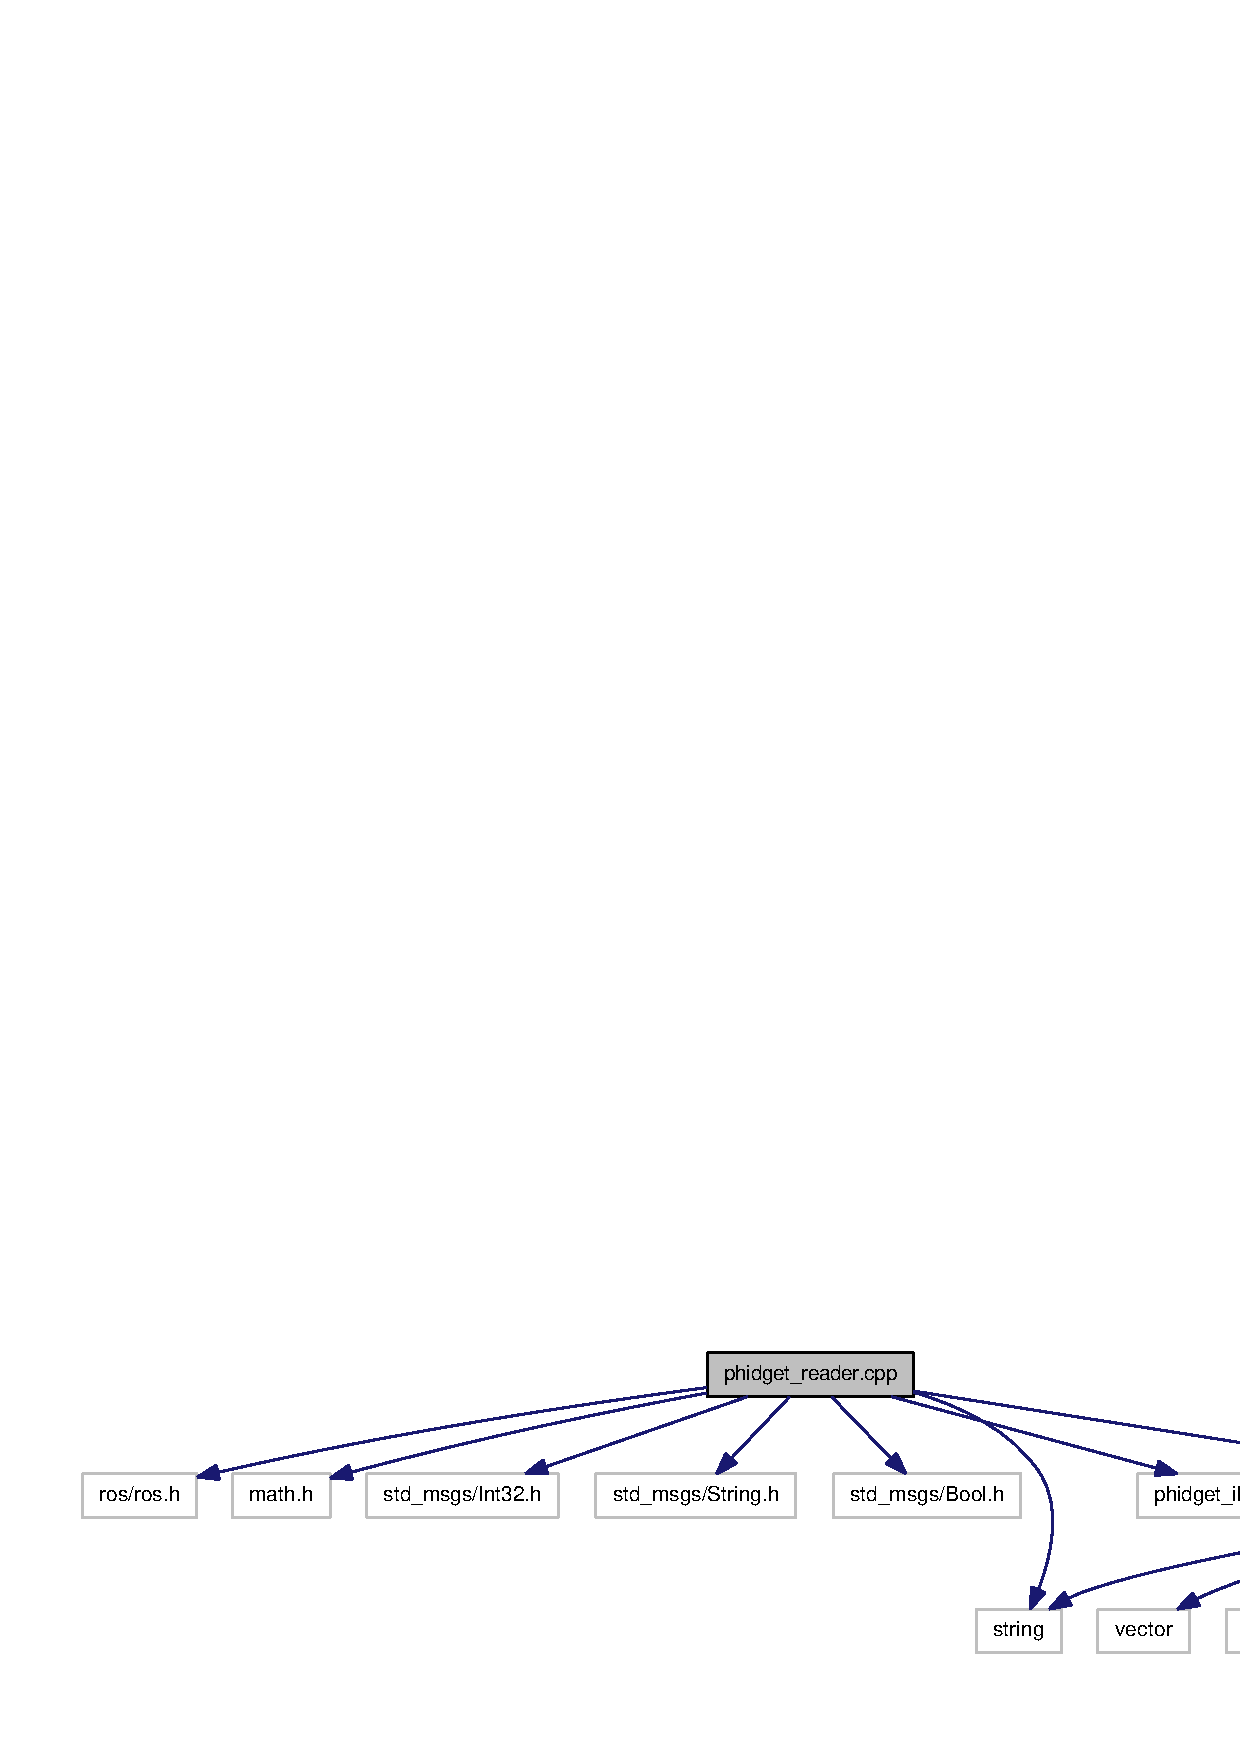
\includegraphics[width=350pt]{phidget__reader_8cpp__incl}
\end{center}
\end{figure}
\subsection*{Functions}
\begin{DoxyCompactItemize}
\item 
int {\bf main} (int argc, char $\ast$$\ast$argv)
\end{DoxyCompactItemize}
\subsection*{Variables}
\begin{DoxyCompactItemize}
\item 
int {\bf sensor\-\_\-id} = 0
\end{DoxyCompactItemize}


\subsection{Function Documentation}
\index{phidget\-\_\-reader.\-cpp@{phidget\-\_\-reader.\-cpp}!main@{main}}
\index{main@{main}!phidget_reader.cpp@{phidget\-\_\-reader.\-cpp}}
\subsubsection[{main}]{\setlength{\rightskip}{0pt plus 5cm}int main (
\begin{DoxyParamCaption}
\item[{int}]{argc, }
\item[{char $\ast$$\ast$}]{argv}
\end{DoxyParamCaption}
)}\label{phidget__reader_8cpp_a3c04138a5bfe5d72780bb7e82a18e627}


Definition at line 8 of file phidget\-\_\-reader.\-cpp.



\subsection{Variable Documentation}
\index{phidget\-\_\-reader.\-cpp@{phidget\-\_\-reader.\-cpp}!sensor\-\_\-id@{sensor\-\_\-id}}
\index{sensor\-\_\-id@{sensor\-\_\-id}!phidget_reader.cpp@{phidget\-\_\-reader.\-cpp}}
\subsubsection[{sensor\-\_\-id}]{\setlength{\rightskip}{0pt plus 5cm}int sensor\-\_\-id = 0}\label{phidget__reader_8cpp_a1b83cf3bbc9916bc2a4d0e75ba23b9d3}


Definition at line 6 of file phidget\-\_\-reader.\-cpp.


\section{rviz\-\_\-gripper.\-cpp File Reference}
\label{rviz__gripper_8cpp}\index{rviz\-\_\-gripper.\-cpp@{rviz\-\_\-gripper.\-cpp}}
{\ttfamily \#include $<$ros/ros.\-h$>$}\\*
{\ttfamily \#include $<$string$>$}\\*
{\ttfamily \#include $<$std\-\_\-msgs/\-Float32.\-h$>$}\\*
{\ttfamily \#include $<$std\-\_\-msgs/\-Bool.\-h$>$}\\*
{\ttfamily \#include $<$sensor\-\_\-msgs/\-Joint\-State.\-h$>$}\\*
Include dependency graph for rviz\-\_\-gripper.\-cpp\-:\nopagebreak
\begin{figure}[H]
\begin{center}
\leavevmode
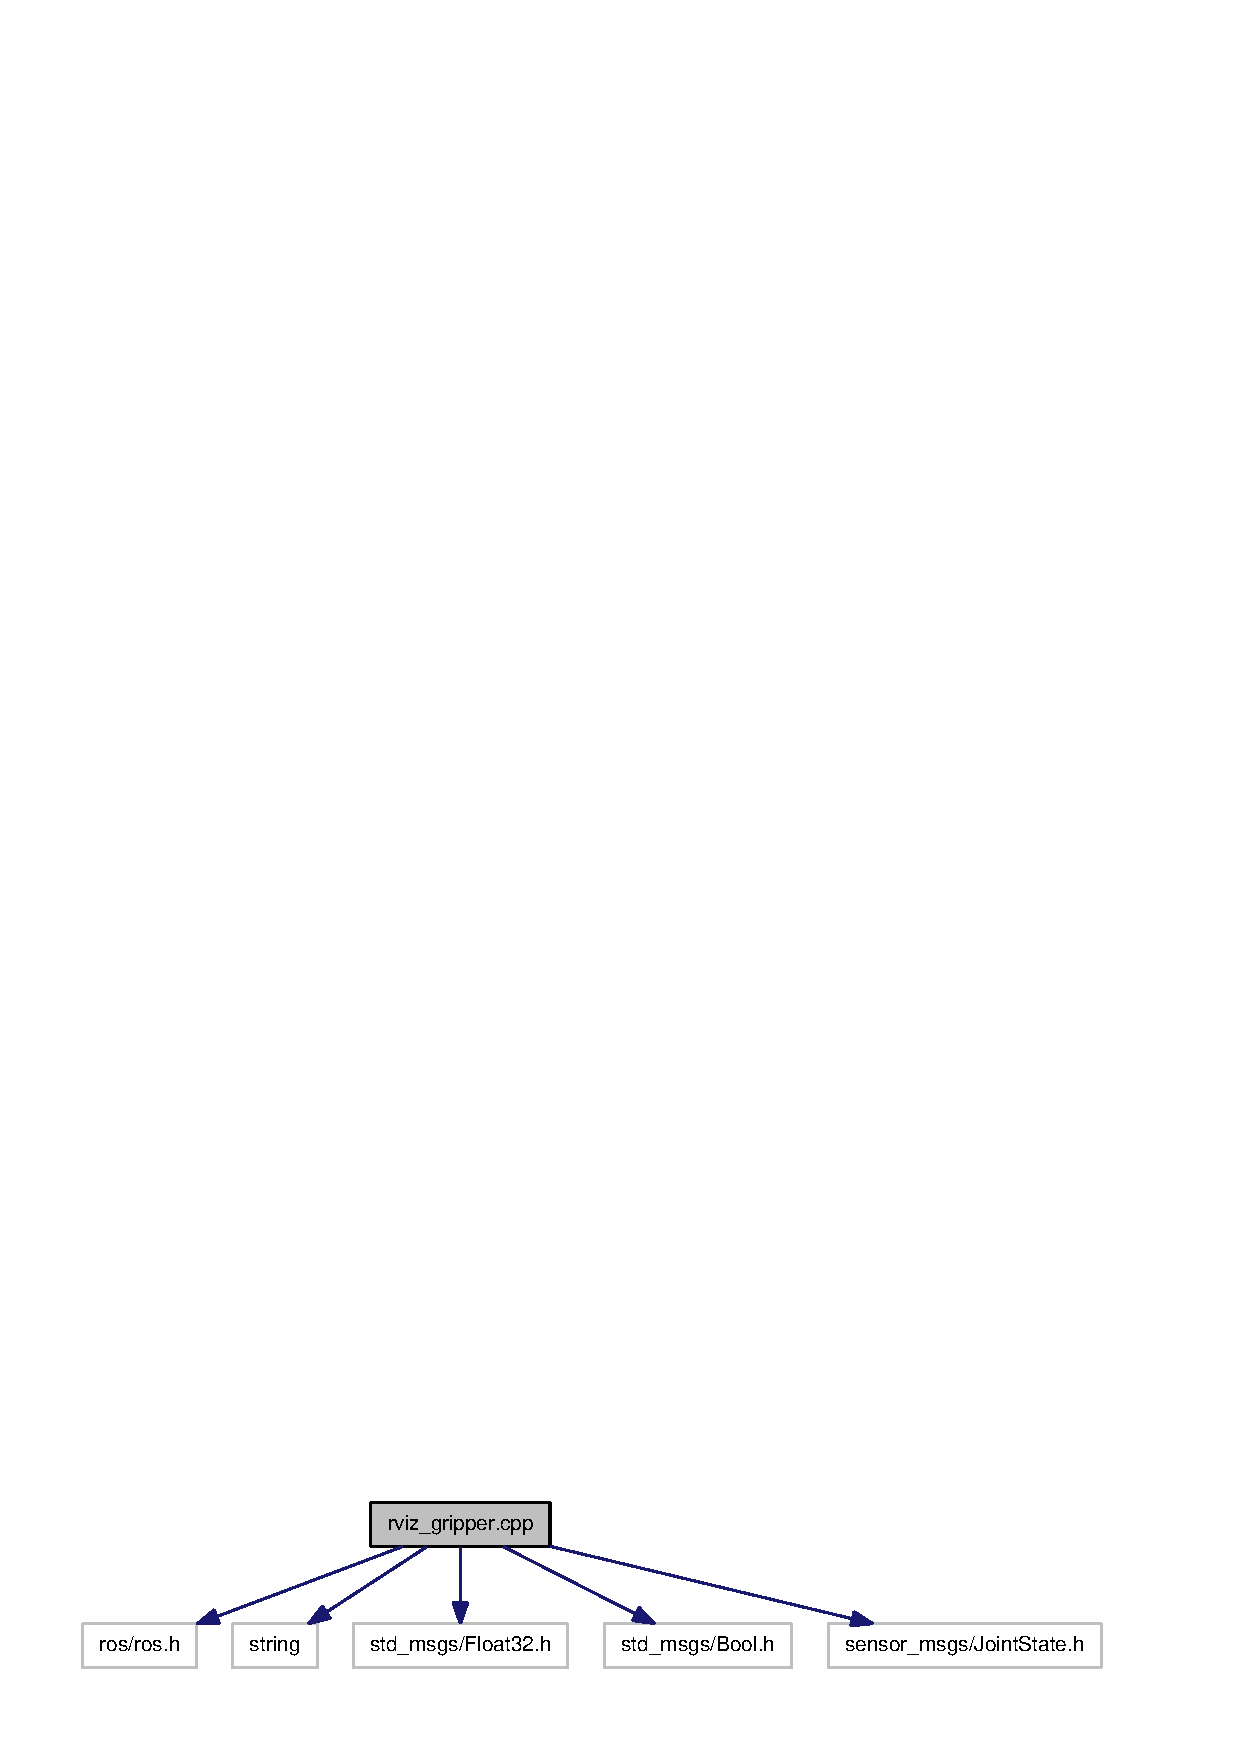
\includegraphics[width=350pt]{rviz__gripper_8cpp__incl}
\end{center}
\end{figure}
\subsection*{Functions}
\begin{DoxyCompactItemize}
\item 
int {\bf main} (int argc, char $\ast$$\ast$argv)
\begin{DoxyCompactList}\small\item\em Main method reads if the state of the gripper is changing and simulates this in R\-V\-I\-Z. \end{DoxyCompactList}\item 
void {\bf rviz\-Updater} (const std\-\_\-msgs\-::\-Float32\-::\-Const\-Ptr \&msg)
\begin{DoxyCompactList}\small\item\em update method the opens variable will be updated \end{DoxyCompactList}\item 
void {\bf shutdown} (const std\-\_\-msgs\-::\-Bool\-::\-Const\-Ptr \&b)
\begin{DoxyCompactList}\small\item\em Controll method to shutdown this R\-O\-S node when the command is given. \end{DoxyCompactList}\end{DoxyCompactItemize}
\subsection*{Variables}
\begin{DoxyCompactItemize}
\item 
const int {\bf freq} = 250
\item 
float {\bf opens}
\end{DoxyCompactItemize}


\subsection{Function Documentation}
\index{rviz\-\_\-gripper.\-cpp@{rviz\-\_\-gripper.\-cpp}!main@{main}}
\index{main@{main}!rviz_gripper.cpp@{rviz\-\_\-gripper.\-cpp}}
\subsubsection[{main}]{\setlength{\rightskip}{0pt plus 5cm}int main (
\begin{DoxyParamCaption}
\item[{int}]{argc, }
\item[{char $\ast$$\ast$}]{argv}
\end{DoxyParamCaption}
)}\label{rviz__gripper_8cpp_a3c04138a5bfe5d72780bb7e82a18e627}


Main method reads if the state of the gripper is changing and simulates this in R\-V\-I\-Z. 

This node listens to the gripper\-\_\-state published by gripper\-\_\-actuator. motor\-\_\-state variable has a value between 1 and 0. 1 means completly open 0 means completly closed. bmdll\-\_\-max angle that the joint between middle and base can make. mlltp\-\_\-max angle that the joint between middle and finger tip can make. bmdll\-\_\-start start angle of the joint between middle and base mdlltp\-\_\-start start angle of the joint between middle and tip bm\-\_\-angle current angle between base and middle mt\-\_\-angle current angle between middle and tip step\-\_\-size the change of motor\-\_\-state per loop cf corection facter the factor the raid at which the tip moves faster then the middle part angle\-\_\-step the inverse of the total angle that can be made by the two joints

The motor\-\_\-state is only changed if the gripper opens or closes and the motor state is between 1 and 0 The new motor\-\_\-state is converted to angles for the both joints. The new angles will be published in the jstates topic

\begin{DoxySeeAlso}{See Also}
\doxyref{shift\-Buffer(int)}{p.}{phidget__reader_8cpp_ab3f7db7de2a2af54619cd7ac3517b924}, \doxyref{mean()}{p.}{phidget__reader_8cpp_a478ef96a3ad4032e1f91152178c8809e} 
\end{DoxySeeAlso}


Definition at line 36 of file rviz\-\_\-gripper.\-cpp.

\index{rviz\-\_\-gripper.\-cpp@{rviz\-\_\-gripper.\-cpp}!rviz\-Updater@{rviz\-Updater}}
\index{rviz\-Updater@{rviz\-Updater}!rviz_gripper.cpp@{rviz\-\_\-gripper.\-cpp}}
\subsubsection[{rviz\-Updater}]{\setlength{\rightskip}{0pt plus 5cm}void rviz\-Updater (
\begin{DoxyParamCaption}
\item[{const std\-\_\-msgs\-::\-Float32\-::\-Const\-Ptr \&}]{msg}
\end{DoxyParamCaption}
)}\label{rviz__gripper_8cpp_ac3a597a9b78812a52a356d6112ebe8f6}


update method the opens variable will be updated 

Method for publishing a cylinder in rviz.


\begin{DoxyParams}{Parameters}
{\em msg} & contains the value 0,1,0.\-5 depending if the gripper is openening, closing or relaxing.\\
\hline
\end{DoxyParams}
This Method creates a marker message to create a cylinder in rviz. The frame where the marker in will be plotted in rviz is the base frame of the gripper. The marker will be deleted if there is no object in the range of the sensor. The type of the marker is a cylinder. Marker will be placed on the y-\/axis on the measured distance from the origin The size of the marker is determined with the diameter and height variable. The color of the marker is green. 

Definition at line 97 of file rviz\-\_\-gripper.\-cpp.

\index{rviz\-\_\-gripper.\-cpp@{rviz\-\_\-gripper.\-cpp}!shutdown@{shutdown}}
\index{shutdown@{shutdown}!rviz_gripper.cpp@{rviz\-\_\-gripper.\-cpp}}
\subsubsection[{shutdown}]{\setlength{\rightskip}{0pt plus 5cm}void shutdown (
\begin{DoxyParamCaption}
\item[{const std\-\_\-msgs\-::\-Bool\-::\-Const\-Ptr \&}]{b}
\end{DoxyParamCaption}
)}\label{rviz__gripper_8cpp_a6099bcde46c020c0703be2c28a4432d5}


Controll method to shutdown this R\-O\-S node when the command is given. 

This method will shutdown this node when the command is given by the console. 
\begin{DoxyParams}{Parameters}
{\em b} & The message containing the command. Nothing is done with the command since we know what it will be when this message is received. \\
\hline
\end{DoxyParams}


\subsection{Variable Documentation}
\index{rviz\-\_\-gripper.\-cpp@{rviz\-\_\-gripper.\-cpp}!freq@{freq}}
\index{freq@{freq}!rviz_gripper.cpp@{rviz\-\_\-gripper.\-cpp}}
\subsubsection[{freq}]{\setlength{\rightskip}{0pt plus 5cm}const int freq = 250}\label{rviz__gripper_8cpp_a323a9f2cf2eeae7e0acd9fe48da80fff}
The frequency at which gripper in rviz is updated. 

Definition at line 13 of file rviz\-\_\-gripper.\-cpp.

\index{rviz\-\_\-gripper.\-cpp@{rviz\-\_\-gripper.\-cpp}!opens@{opens}}
\index{opens@{opens}!rviz_gripper.cpp@{rviz\-\_\-gripper.\-cpp}}
\subsubsection[{opens}]{\setlength{\rightskip}{0pt plus 5cm}float opens}\label{rviz__gripper_8cpp_a6593a9dfdfff068cc7a30a1f1ff5000a}
The state of the gripper 0 when gripper closes, 1 when gripper opens, 0.\-5 in relax mode. 

Definition at line 12 of file rviz\-\_\-gripper.\-cpp.


\section{rviz\-\_\-object.\-cpp File Reference}
\label{rviz__object_8cpp}\index{rviz\-\_\-object.\-cpp@{rviz\-\_\-object.\-cpp}}
{\ttfamily \#include $<$ros/ros.\-h$>$}\\*
{\ttfamily \#include $<$string$>$}\\*
{\ttfamily \#include $<$std\-\_\-msgs/\-Int32.\-h$>$}\\*
{\ttfamily \#include $<$std\-\_\-msgs/\-Bool.\-h$>$}\\*
{\ttfamily \#include $<$visualization\-\_\-msgs/\-Marker.\-h$>$}\\*
Include dependency graph for rviz\-\_\-object.\-cpp\-:\nopagebreak
\begin{figure}[H]
\begin{center}
\leavevmode
\includegraphics[width=350pt]{rviz__object_8cpp__incl}
\end{center}
\end{figure}
\subsection*{Functions}
\begin{DoxyCompactItemize}
\item 
int {\bf main} (int argc, char $\ast$$\ast$argv)
\item 
void {\bf rviz\-Updater} (const std\-\_\-msgs\-::\-Int32\-::\-Const\-Ptr \&)
\item 
void {\bf shutdown} (const std\-\_\-msgs\-::\-Bool\-::\-Const\-Ptr \&)
\end{DoxyCompactItemize}
\subsection*{Variables}
\begin{DoxyCompactItemize}
\item 
int {\bf dist\-\_\-int}
\end{DoxyCompactItemize}


\subsection{Function Documentation}
\index{rviz\-\_\-object.\-cpp@{rviz\-\_\-object.\-cpp}!main@{main}}
\index{main@{main}!rviz_object.cpp@{rviz\-\_\-object.\-cpp}}
\subsubsection[{main}]{\setlength{\rightskip}{0pt plus 5cm}int main (
\begin{DoxyParamCaption}
\item[{int}]{argc, }
\item[{char $\ast$$\ast$}]{argv}
\end{DoxyParamCaption}
)}\label{rviz__object_8cpp_a3c04138a5bfe5d72780bb7e82a18e627}


Definition at line 15 of file rviz\-\_\-object.\-cpp.

\index{rviz\-\_\-object.\-cpp@{rviz\-\_\-object.\-cpp}!rviz\-Updater@{rviz\-Updater}}
\index{rviz\-Updater@{rviz\-Updater}!rviz_object.cpp@{rviz\-\_\-object.\-cpp}}
\subsubsection[{rviz\-Updater}]{\setlength{\rightskip}{0pt plus 5cm}void rviz\-Updater (
\begin{DoxyParamCaption}
\item[{const std\-\_\-msgs\-::\-Int32\-::\-Const\-Ptr \&}]{msg}
\end{DoxyParamCaption}
)}\label{rviz__object_8cpp_a9bbd86f31fda8151dd8981cc77d4c21b}


Definition at line 96 of file rviz\-\_\-object.\-cpp.

\index{rviz\-\_\-object.\-cpp@{rviz\-\_\-object.\-cpp}!shutdown@{shutdown}}
\index{shutdown@{shutdown}!rviz_object.cpp@{rviz\-\_\-object.\-cpp}}
\subsubsection[{shutdown}]{\setlength{\rightskip}{0pt plus 5cm}void shutdown (
\begin{DoxyParamCaption}
\item[{const std\-\_\-msgs\-::\-Bool\-::\-Const\-Ptr \&}]{b}
\end{DoxyParamCaption}
)}\label{rviz__object_8cpp_a9eeee6c84a027eabdd7230329be56bec}


\subsection{Variable Documentation}
\index{rviz\-\_\-object.\-cpp@{rviz\-\_\-object.\-cpp}!dist\-\_\-int@{dist\-\_\-int}}
\index{dist\-\_\-int@{dist\-\_\-int}!rviz_object.cpp@{rviz\-\_\-object.\-cpp}}
\subsubsection[{dist\-\_\-int}]{\setlength{\rightskip}{0pt plus 5cm}int dist\-\_\-int}\label{rviz__object_8cpp_a4425b358da5de7e919aa971b57de5504}


Definition at line 13 of file rviz\-\_\-object.\-cpp.


\addcontentsline{toc}{part}{Index}
\printindex
\end{document}
